\begin{figure}
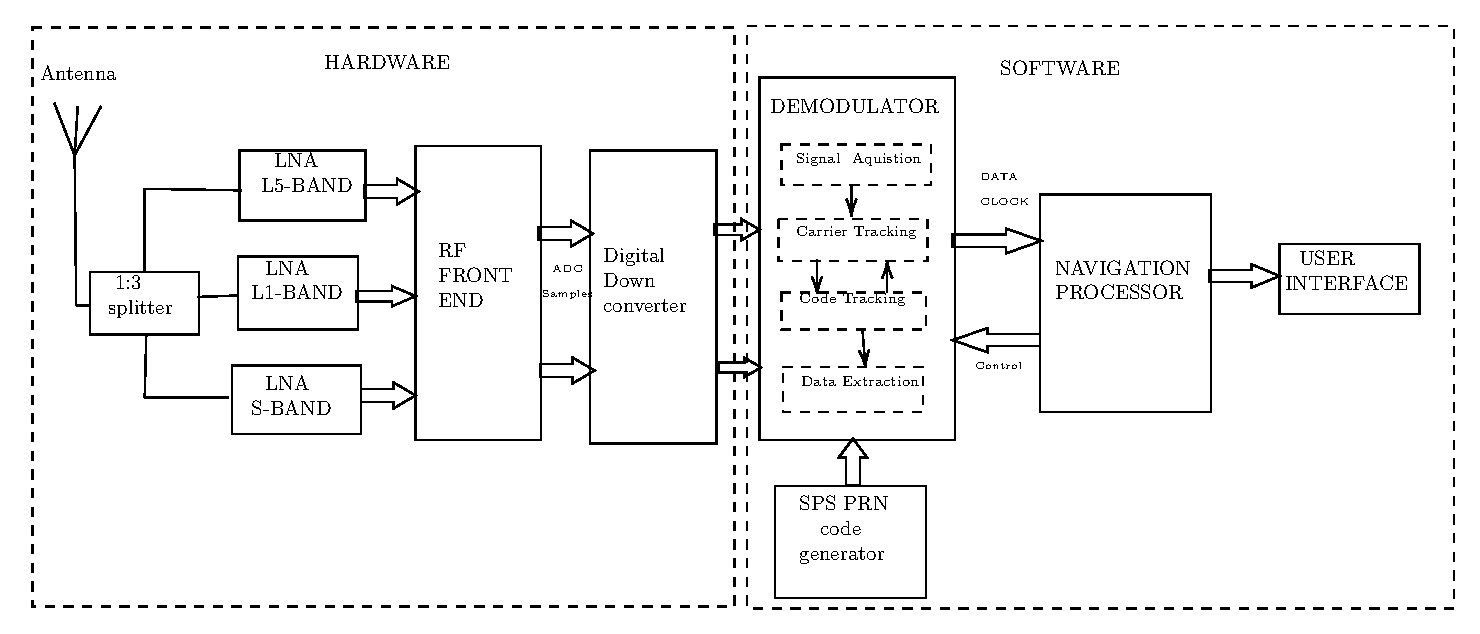
\includegraphics[scale=0.5]{figs/block1}
\caption{The Block Level Architecture}
\label{fig:Block-diagram}
\end{figure}
\section{Hardware Implementation}
\begin{figure}
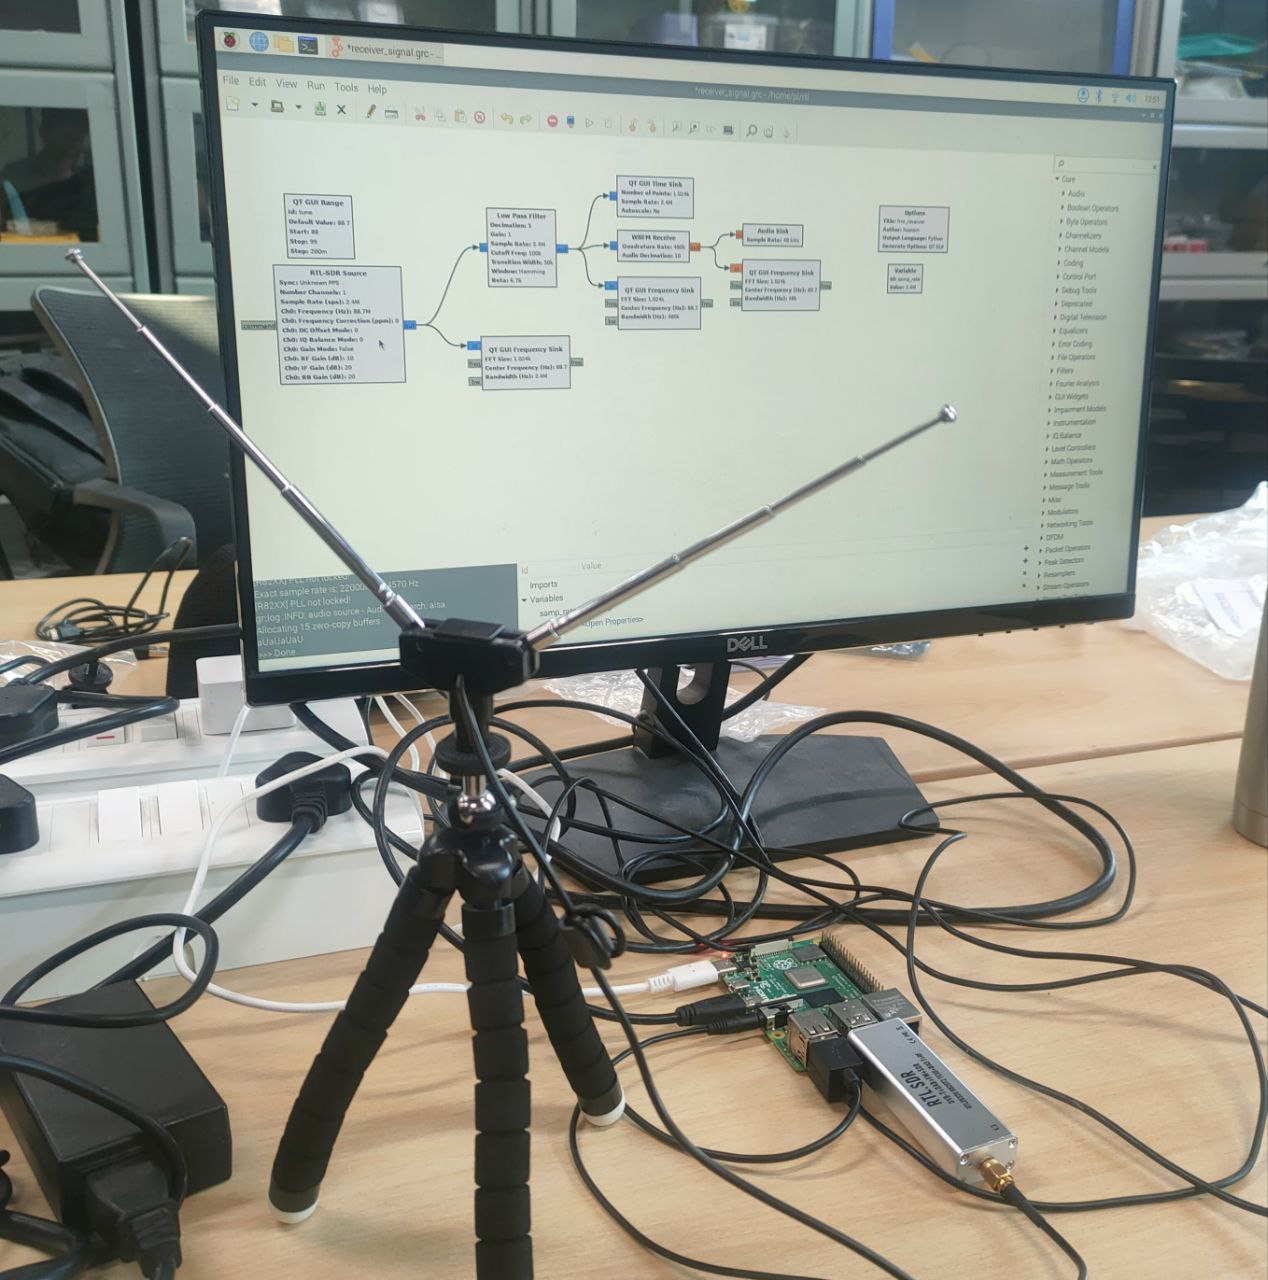
\includegraphics[scale=0.2]{figs/hardwareimplement.jpg} 
\caption{Reciever Hardware implementation}
\label{fig:hardware}
\end{figure}
List the various components used to implement receiver.
\\
\solution
\\
\begin{table}[!ht]
  \centering
 %%%%%%%%%%%%%%%%%%%%%%%%%%%%%%%%%%%%%%%%%%%%%%%%%%%%%%%%%%%%%%%%%%%%%%
%%                                                                  %%
%%  This is the header of a LaTeX2e file exported from Gnumeric.    %%
%%                                                                  %%
%%  This file can be compiled as it stands or included in another   %%
%%  LaTeX document. The table is based on the longtable package so  %%
%%  the longtable options (headers, footers...) can be set in the   %%
%%  preamble section below (see PRAMBLE).                           %%
%%                                                                  %%
%%  To include the file in another, the following two lines must be %%
%%  in the including file:                                          %%
%%        \def\inputGnumericTable{}                                 %%
%%  at the beginning of the file and:                               %%
%%        \input{name-of-this-file.tex}                             %%
%%  where the table is to be placed. Note also that the including   %%
%%  file must use the following packages for the table to be        %%
%%  rendered correctly:                                             %%
%%    \usepackage[latin1]{inputenc}                                 %%
%%    \usepackage{color}                                            %%
%%    \usepackage{array}                                            %%
%%    \usepackage{longtable}                                        %%
%%    \usepackage{calc}                                             %%
%%    \usepackage{multirow}                                         %%
%%    \usepackage{hhline}                                           %%
%%    \usepackage{ifthen}                                           %%
%%  optionally (for landscape tables embedded in another document): %%
%%    \usepackage{lscape}                                           %%
%%                                                                  %%
%%%%%%%%%%%%%%%%%%%%%%%%%%%%%%%%%%%%%%%%%%%%%%%%%%%%%%%%%%%%%%%%%%%%%%



%%  This section checks if we are begin input into another file or  %%
%%  the file will be compiled alone. First use a macro taken from   %%
%%  the TeXbook ex 7.7 (suggestion of Han-Wen Nienhuys).            %%
\def\ifundefined#1{\expandafter\ifx\csname#1\endcsname\relax}


%%  Check for the \def token for inputed files. If it is not        %%
%%  defined, the file will be processed as a standalone and the     %%
%%  preamble will be used.                                          %%
\ifundefined{inputGnumericTable}

%%  We must be able to close or not the document at the end.        %%
	\def\gnumericTableEnd{\end{document}}


%%%%%%%%%%%%%%%%%%%%%%%%%%%%%%%%%%%%%%%%%%%%%%%%%%%%%%%%%%%%%%%%%%%%%%
%%                                                                  %%
%%  This is the PREAMBLE. Change these values to get the right      %%
%%  paper size and other niceties.                                  %%
%%                                                                  %%
%%%%%%%%%%%%%%%%%%%%%%%%%%%%%%%%%%%%%%%%%%%%%%%%%%%%%%%%%%%%%%%%%%%%%%

	\documentclass[12pt%
			  %,landscape%
                    ]{report}
       \usepackage[latin1]{inputenc}
       \usepackage{fullpage}
       \usepackage{color}
       \usepackage{array}
       \usepackage{longtable}
       \usepackage{calc}
       \usepackage{multirow}
       \usepackage{hhline}
       \usepackage{ifthen}

	\begin{document}


%%  End of the preamble for the standalone. The next section is for %%
%%  documents which are included into other LaTeX2e files.          %%
\else

%%  We are not a stand alone document. For a regular table, we will %%
%%  have no preamble and only define the closing to mean nothing.   %%
    \def\gnumericTableEnd{}

%%  If we want landscape mode in an embedded document, comment out  %%
%%  the line above and uncomment the two below. The table will      %%
%%  begin on a new page and run in landscape mode.                  %%
%       \def\gnumericTableEnd{\end{landscape}}
%       \begin{landscape}


%%  End of the else clause for this file being \input.              %%
\fi

%%%%%%%%%%%%%%%%%%%%%%%%%%%%%%%%%%%%%%%%%%%%%%%%%%%%%%%%%%%%%%%%%%%%%%
%%                                                                  %%
%%  The rest is the gnumeric table, except for the closing          %%
%%  statement. Changes below will alter the table's appearance.     %%
%%                                                                  %%
%%%%%%%%%%%%%%%%%%%%%%%%%%%%%%%%%%%%%%%%%%%%%%%%%%%%%%%%%%%%%%%%%%%%%%

\providecommand{\gnumericmathit}[1]{#1} 
%%  Uncomment the next line if you would like your numbers to be in %%
%%  italics if they are italizised in the gnumeric table.           %%
%\renewcommand{\gnumericmathit}[1]{\mathit{#1}}
\providecommand{\gnumericPB}[1]%
{\let\gnumericTemp=\\#1\let\\=\gnumericTemp\hspace{0pt}}
 \ifundefined{gnumericTableWidthDefined}
        \newlength{\gnumericTableWidth}
        \newlength{\gnumericTableWidthComplete}
        \newlength{\gnumericMultiRowLength}
        \global\def\gnumericTableWidthDefined{}
 \fi
%% The following setting protects this code from babel shorthands.  %%
 \ifthenelse{\isundefined{\languageshorthands}}{}{\languageshorthands{english}}
%%  The default table format retains the relative column widths of  %%
%%  gnumeric. They can easily be changed to c, r or l. In that case %%
%%  you may want to comment out the next line and uncomment the one %%
%%  thereafter                                                      %%
\providecommand\gnumbox{\makebox[0pt]}
%%\providecommand\gnumbox[1][]{\makebox}

%% to adjust positions in multirow situations                       %%
\setlength{\bigstrutjot}{\jot}
\setlength{\extrarowheight}{\doublerulesep}

%%  The \setlongtables command keeps column widths the same across  %%
%%  pages. Simply comment out next line for varying column widths.  %%
\setlongtables

\setlength\gnumericTableWidth{%
	98pt+%
	215pt+%
	53pt+%
	53pt+%
0pt}
\def\gumericNumCols{4}
\setlength\gnumericTableWidthComplete{\gnumericTableWidth+%
         \tabcolsep*\gumericNumCols*2+\arrayrulewidth*\gumericNumCols}
\ifthenelse{\lengthtest{\gnumericTableWidthComplete > \linewidth}}%
         {\def\gnumericScale{1*\ratio{\linewidth-%
                        \tabcolsep*\gumericNumCols*2-%
                        \arrayrulewidth*\gumericNumCols}%
{\gnumericTableWidth}}}%
{\def\gnumericScale{1}}

%%%%%%%%%%%%%%%%%%%%%%%%%%%%%%%%%%%%%%%%%%%%%%%%%%%%%%%%%%%%%%%%%%%%%%
%%                                                                  %%
%% The following are the widths of the various columns. We are      %%
%% defining them here because then they are easier to change.       %%
%% Depending on the cell formats we may use them more than once.    %%
%%                                                                  %%
%%%%%%%%%%%%%%%%%%%%%%%%%%%%%%%%%%%%%%%%%%%%%%%%%%%%%%%%%%%%%%%%%%%%%%

\ifthenelse{\isundefined{\gnumericColA}}{\newlength{\gnumericColA}}{}\settowidth{\gnumericColA}{\begin{tabular}{@{}p{98pt*\gnumericScale}@{}}x\end{tabular}}
\ifthenelse{\isundefined{\gnumericColB}}{\newlength{\gnumericColB}}{}\settowidth{\gnumericColB}{\begin{tabular}{@{}p{215pt*\gnumericScale}@{}}x\end{tabular}}
\ifthenelse{\isundefined{\gnumericColC}}{\newlength{\gnumericColC}}{}\settowidth{\gnumericColC}{\begin{tabular}{@{}p{53pt*\gnumericScale}@{}}x\end{tabular}}
\ifthenelse{\isundefined{\gnumericColD}}{\newlength{\gnumericColD}}{}\settowidth{\gnumericColD}{\begin{tabular}{@{}p{53pt*\gnumericScale}@{}}x\end{tabular}}

\begin{longtable}[c]{%
	b{\gnumericColA}%
	b{\gnumericColB}%
	b{\gnumericColC}%
	b{\gnumericColD}%
	}

%%%%%%%%%%%%%%%%%%%%%%%%%%%%%%%%%%%%%%%%%%%%%%%%%%%%%%%%%%%%%%%%%%%%%%
%%  The longtable options. (Caption, headers... see Goosens, p.124) %%
%	\caption{The Table Caption.}             \\	%
% \hline	% Across the top of the table.
%%  The rest of these options are table rows which are placed on    %%
%%  the first, last or every page. Use \multicolumn if you want.    %%

%%  Header for the first page.                                      %%
%	\multicolumn{4}{c}{The First Header} \\ \hline 
%	\multicolumn{1}{c}{colTag}	%Column 1
%	&\multicolumn{1}{c}{colTag}	%Column 2
%	&\multicolumn{1}{c}{colTag}	%Column 3
%	&\multicolumn{1}{c}{colTag}	\\ \hline %Last column
%	\endfirsthead

%%  The running header definition.                                  %%
%	\hline
%	\multicolumn{4}{l}{\ldots\small\slshape continued} \\ \hline
%	\multicolumn{1}{c}{colTag}	%Column 1
%	&\multicolumn{1}{c}{colTag}	%Column 2
%	&\multicolumn{1}{c}{colTag}	%Column 3
%	&\multicolumn{1}{c}{colTag}	\\ \hline %Last column
%	\endhead

%%  The running footer definition.                                  %%
%	\hline
%	\multicolumn{4}{r}{\small\slshape continued\ldots} \\
%	\endfoot

%%  The ending footer definition.                                   %%
%	\multicolumn{4}{c}{That's all folks} \\ \hline 
%	\endlastfoot
%%%%%%%%%%%%%%%%%%%%%%%%%%%%%%%%%%%%%%%%%%%%%%%%%%%%%%%%%%%%%%%%%%%%%%

\hhline{|-|-|--}
	 \multicolumn{1}{|p{\gnumericColA}|}%
	{\gnumericPB{\centering}\gnumbox{\textbf{Component}}}
	&\multicolumn{1}{p{\gnumericColB}|}%
	{\gnumericPB{\centering}\gnumbox{\textbf{Type}}}
	
\\
\hhline{|----|}
	 \multicolumn{1}{|p{\gnumericColA}|}%
	{\gnumericPB{\centering}\gnumbox{RTL-SDR chip}}
	&\multicolumn{1}{p{\gnumericColB}|}%
	{\gnumericPB{\raggedright}\gnumbox[l]{Hardware}}
	
\\
\hhline{|----|}
	 \multicolumn{1}{|p{\gnumericColA}|}%
	{\gnumericPB{\centering}\gnumbox{GNU radio}}
	&\multicolumn{1}{p{\gnumericColB}|}%
	{\gnumericPB{\raggedright}\gnumbox[l]{Software}}
	
\\
\hhline{|----|}
	 \multicolumn{1}{|p{\gnumericColA}|}%
	{\gnumericPB{\centering}\gnumbox{Antenna}}
	&\multicolumn{1}{p{\gnumericColB}|}%
	{\gnumericPB{\raggedright}\gnumbox[l]{Hardware}}
	

\\
\hhline{|-|-|--|}
\end{longtable}

\ifthenelse{\isundefined{\languageshorthands}}{}{\languageshorthands{\languagename}}
\gnumericTableEnd

  \caption{Components Required}
  \label{tab:rxcomponents}
\end{table}
Components are listed in the table \tabref{tab:rxcomponents}\\
The picture of RTL-SDR and Antenna is given in \figref{fig:hardware}.This set is used to receive the L5,L1,S Band  signals.
\begin{figure}[ht]
\centering
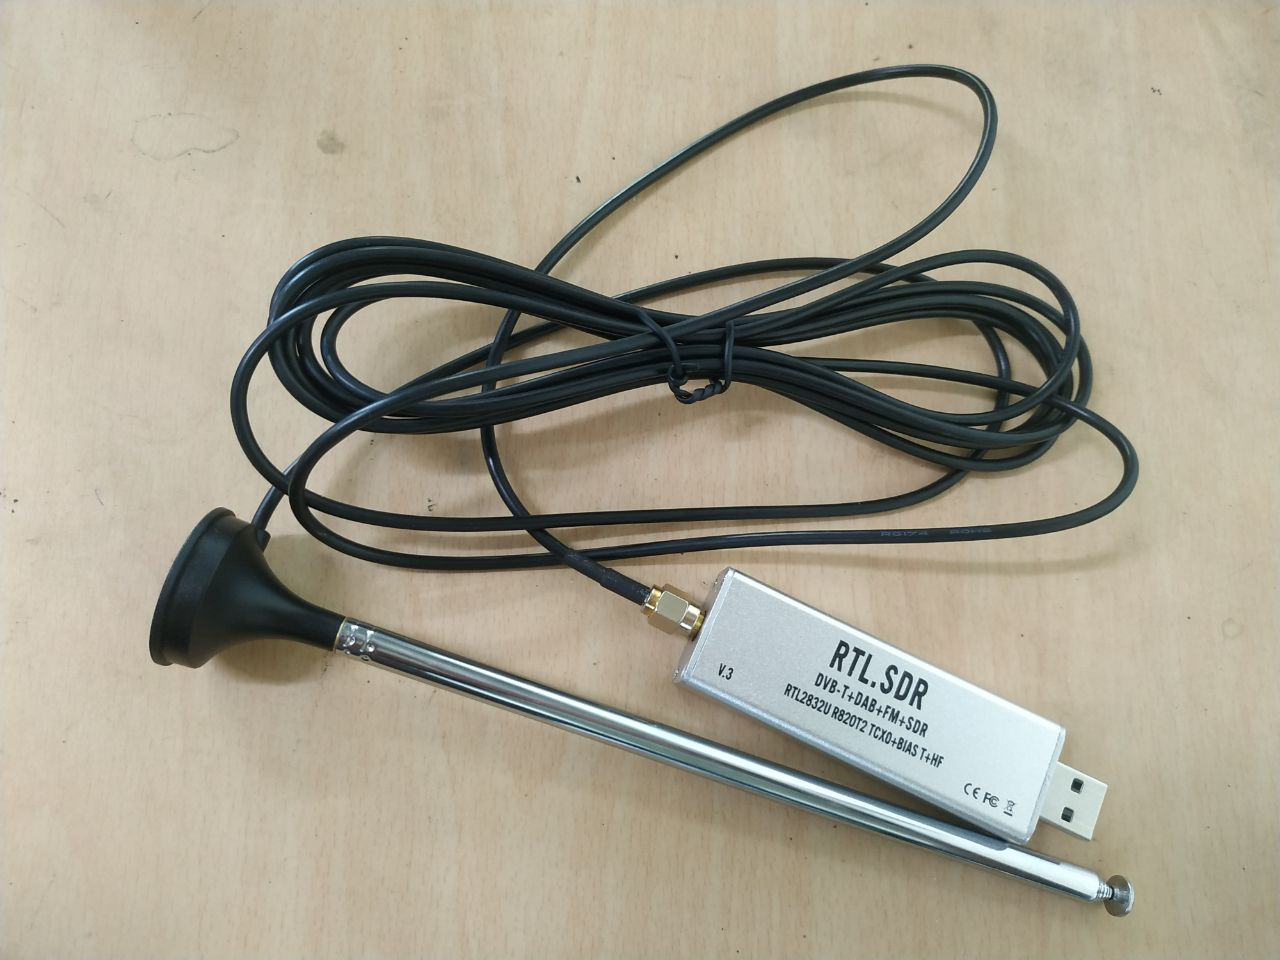
\includegraphics[width=0.5\columnwidth]{figs/rtl-sdr.png}
\caption{RTL-SDR}
\label{fig:rtl-sdr}
\end{figure}
\section{RTL SDR Specifications}
RTL-SDR is a popular, low cost hardware that can receive wireless signals. The RTL-SDR dongle features the Realtek RTL2838U chip, which provides I-Q samples through the USB interface. 
\begin{table}[!ht]
  \centering
 %%%%%%%%%%%%%%%%%%%%%%%%%%%%%%%%%%%%%%%%%%%%%%%%%%%%%%%%%%%%%%%%%%%%%%
%%                                                                  %%
%%  This is the header of a LaTeX2e file exported from Gnumeric.    %%
%%                                                                  %%
%%  This file can be compiled as it stands or included in another   %%
%%  LaTeX document. The table is based on the longtable package so  %%
%%  the longtable options (headers, footers...) can be set in the   %%
%%  preamble section below (see PRAMBLE).                           %%
%%                                                                  %%
%%  To include the file in another, the following two lines must be %%
%%  in the including file:                                          %%
%%        \def\inputGnumericTable{}                                 %%
%%  at the beginning of the file and:                               %%
%%        \input{name-of-this-file.tex}                             %%
%%  where the table is to be placed. Note also that the including   %%
%%  file must use the following packages for the table to be        %%
%%  rendered correctly:                                             %%
%%    \usepackage[latin1]{inputenc}                                 %%
%%    \usepackage{color}                                            %%
%%    \usepackage{array}                                            %%
%%    \usepackage{longtable}                                        %%
%%    \usepackage{calc}                                             %%
%%    \usepackage{multirow}                                         %%
%%    \usepackage{hhline}                                           %%
%%    \usepackage{ifthen}                                           %%
%%  optionally (for landscape tables embedded in another document): %%
%%    \usepackage{lscape}                                           %%
%%                                                                  %%
%%%%%%%%%%%%%%%%%%%%%%%%%%%%%%%%%%%%%%%%%%%%%%%%%%%%%%%%%%%%%%%%%%%%%%



%%  This section checks if we are begin input into another file or  %%
%%  the file will be compiled alone. First use a macro taken from   %%
%%  the TeXbook ex 7.7 (suggestion of Han-Wen Nienhuys).            %%
\def\ifundefined#1{\expandafter\ifx\csname#1\endcsname\relax}


%%  Check for the \def token for inputed files. If it is not        %%
%%  defined, the file will be processed as a standalone and the     %%
%%  preamble will be used.                                          %%
\ifundefined{inputGnumericTable}

%%  We must be able to close or not the document at the end.        %%
	\def\gnumericTableEnd{\end{document}}


%%%%%%%%%%%%%%%%%%%%%%%%%%%%%%%%%%%%%%%%%%%%%%%%%%%%%%%%%%%%%%%%%%%%%%
%%                                                                  %%
%%  This is the PREAMBLE. Change these values to get the right      %%
%%  paper size and other niceties.                                  %%
%%                                                                  %%
%%%%%%%%%%%%%%%%%%%%%%%%%%%%%%%%%%%%%%%%%%%%%%%%%%%%%%%%%%%%%%%%%%%%%%

	\documentclass[12pt%
			  %,landscape%
                    ]{report}
       \usepackage[latin1]{inputenc}
       \usepackage{fullpage}
       \usepackage{color}
       \usepackage{array}
       \usepackage{longtable}
       \usepackage{calc}
       \usepackage{multirow}
       \usepackage{hhline}
       \usepackage{ifthen}

	\begin{document}


%%  End of the preamble for the standalone. The next section is for %%
%%  documents which are included into other LaTeX2e files.          %%
\else

%%  We are not a stand alone document. For a regular table, we will %%
%%  have no preamble and only define the closing to mean nothing.   %%
    \def\gnumericTableEnd{}

%%  If we want landscape mode in an embedded document, comment out  %%
%%  the line above and uncomment the two below. The table will      %%
%%  begin on a new page and run in landscape mode.                  %%
%       \def\gnumericTableEnd{\end{landscape}}
%       \begin{landscape}


%%  End of the else clause for this file being \input.              %%
\fi

%%%%%%%%%%%%%%%%%%%%%%%%%%%%%%%%%%%%%%%%%%%%%%%%%%%%%%%%%%%%%%%%%%%%%%
%%                                                                  %%
%%  The rest is the gnumeric table, except for the closing          %%
%%  statement. Changes below will alter the table's appearance.     %%
%%                                                                  %%
%%%%%%%%%%%%%%%%%%%%%%%%%%%%%%%%%%%%%%%%%%%%%%%%%%%%%%%%%%%%%%%%%%%%%%

\providecommand{\gnumericmathit}[1]{#1} 
%%  Uncomment the next line if you would like your numbers to be in %%
%%  italics if they are italizised in the gnumeric table.           %%
%\renewcommand{\gnumericmathit}[1]{\mathit{#1}}
\providecommand{\gnumericPB}[1]%
{\let\gnumericTemp=\\#1\let\\=\gnumericTemp\hspace{0pt}}
 \ifundefined{gnumericTableWidthDefined}
        \newlength{\gnumericTableWidth}
        \newlength{\gnumericTableWidthComplete}
        \newlength{\gnumericMultiRowLength}
        \global\def\gnumericTableWidthDefined{}
 \fi
%% The following setting protects this code from babel shorthands.  %%
 \ifthenelse{\isundefined{\languageshorthands}}{}{\languageshorthands{english}}
%%  The default table format retains the relative column widths of  %%
%%  gnumeric. They can easily be changed to c, r or l. In that case %%
%%  you may want to comment out the next line and uncomment the one %%
%%  thereafter                                                      %%
\providecommand\gnumbox{\makebox[0pt]}
%%\providecommand\gnumbox[1][]{\makebox}

%% to adjust positions in multirow situations                       %%
\setlength{\bigstrutjot}{\jot}
\setlength{\extrarowheight}{\doublerulesep}

%%  The \setlongtables command keeps column widths the same across  %%
%%  pages. Simply comment out next line for varying column widths.  %%
\setlongtables

\setlength\gnumericTableWidth{%
	95pt+%
	235pt+%
0pt}
\def\gumericNumCols{2}
\setlength\gnumericTableWidthComplete{\gnumericTableWidth+%
         \tabcolsep*\gumericNumCols*2+\arrayrulewidth*\gumericNumCols}
\ifthenelse{\lengthtest{\gnumericTableWidthComplete > \linewidth}}%
         {\def\gnumericScale{\ratio{\linewidth-%
                        \tabcolsep*\gumericNumCols*2-%
                        \arrayrulewidth*\gumericNumCols}%
{\gnumericTableWidth}}}%
{\def\gnumericScale{1}}

%%%%%%%%%%%%%%%%%%%%%%%%%%%%%%%%%%%%%%%%%%%%%%%%%%%%%%%%%%%%%%%%%%%%%%
%%                                                                  %%
%% The following are the widths of the various columns. We are      %%
%% defining them here because then they are easier to change.       %%
%% Depending on the cell formats we may use them more than once.    %%
%%                                                                  %%
%%%%%%%%%%%%%%%%%%%%%%%%%%%%%%%%%%%%%%%%%%%%%%%%%%%%%%%%%%%%%%%%%%%%%%

\ifthenelse{\isundefined{\gnumericColA}}{\newlength{\gnumericColA}}{}\settowidth{\gnumericColA}{\begin{tabular}{@{}p{95pt*\gnumericScale}@{}}x\end{tabular}}
\ifthenelse{\isundefined{\gnumericColB}}{\newlength{\gnumericColB}}{}\settowidth{\gnumericColB}{\begin{tabular}{@{}p{235pt*\gnumericScale}@{}}x\end{tabular}}

\begin{longtable}[c]{%
	b{\gnumericColA}%
	b{\gnumericColB}%
	}

%%%%%%%%%%%%%%%%%%%%%%%%%%%%%%%%%%%%%%%%%%%%%%%%%%%%%%%%%%%%%%%%%%%%%%
%%  The longtable options. (Caption, headers... see Goosens, p.124) %%
%	\caption{The Table Caption.}             \\	%
% \hline	% Across the top of the table.
%%  The rest of these options are table rows which are placed on    %%
%%  the first, last or every page. Use \multicolumn if you want.    %%

%%  Header for the first page.                                      %%
%	\multicolumn{2}{c}{The First Header} \\ \hline 
%	\multicolumn{1}{c}{colTag}	%Column 1
%	&\multicolumn{1}{c}{colTag}	\\ \hline %Last column
%	\endfirsthead

%%  The running header definition.                                  %%
%	\hline
%	\multicolumn{2}{l}{\ldots\small\slshape continued} \\ \hline
%	\multicolumn{1}{c}{colTag}	%Column 1
%	&\multicolumn{1}{c}{colTag}	\\ \hline %Last column
%	\endhead

%%  The running footer definition.                                  %%
%	\hline
%	\multicolumn{2}{r}{\small\slshape continued\ldots} \\
%	\endfoot

%%  The ending footer definition.                                   %%
%	\multicolumn{2}{c}{That's all folks} \\ \hline 
%	\endlastfoot
%%%%%%%%%%%%%%%%%%%%%%%%%%%%%%%%%%%%%%%%%%%%%%%%%%%%%%%%%%%%%%%%%%%%%%

\hhline{|-|-}
	 \multicolumn{1}{|p{\gnumericColA}|}%
	{\gnumericPB{\raggedright}\gnumbox[l]{\hspace{0.75cm}\textbf{Name}}}
	&\multicolumn{1}{p{\gnumericColB}|}%
	{\gnumericPB{\raggedright}\gnumbox[l]{ \textbf{RTL-SDR(R820T2/RTL2838U DVB-T)}}}
\\
\hhline{|--|}
	 \multicolumn{1}{|p{\gnumericColA}|}%
	{\gnumericPB{\raggedright}\gnumbox[l]{Type}}
	&\multicolumn{1}{p{\gnumericColB}|}%
	{\gnumericPB{\raggedright}\gnumbox[l]{Pre-built and premodded with custom driver}}
\\
\hhline{|--|}
	 \multicolumn{1}{|p{\gnumericColA}|}%
	{\gnumericPB{\raggedright}\gnumbox[l]{Frequency range}}
	&\multicolumn{1}{p{\gnumericColB}|}%
	{\gnumericPB{\raggedright}\gnumbox[l]{0.5-1766MHz}}
\\
\hhline{|--|}
	 \multicolumn{1}{|p{\gnumericColA}|}%
	{\gnumericPB{\raggedright}\gnumbox[l]{Max Bandwidth}}
	&\multicolumn{1}{p{\gnumericColB}|}%
	{\gnumericPB{\raggedright}\gnumbox[l]{Matches sampling rate but with filter roll-off}}
\\
\hhline{|--|}
	 \multicolumn{1}{|p{\gnumericColA}|}%
	{\gnumericPB{\raggedright}\gnumbox[l]{Receiver ADC bits }}
	&\multicolumn{1}{p{\gnumericColB}|}%
	{\gnumericPB{\raggedright}\gnumbox[l]{8}}
\\
\hhline{|--|}
	 \multicolumn{1}{|p{\gnumericColA}|}%
	{\gnumericPB{\raggedright}\gnumbox[l]{Tx.DAC bits}}
	&\multicolumn{1}{p{\gnumericColB}|}%
	{\gnumericPB{\raggedright}\gnumbox[l]{-}}
\\
\hhline{|--|}
	 \multicolumn{1}{|p{\gnumericColA}|}%
	{\gnumericPB{\raggedright}\gnumbox[l]{Tx. Cable }}
	&\multicolumn{1}{p{\gnumericColB}|}%
	{\gnumericPB{\raggedright}\gnumbox[l]{No}}
\\
\hhline{|--|}
	 \multicolumn{1}{|p{\gnumericColA}|}%
	{\gnumericPB{\raggedright}\gnumbox[l]{Sampling Rate }}
	&\multicolumn{1}{p{\gnumericColB}|}%
	{\gnumericPB{\raggedright}\gnumbox[l]{2.4 MHz }}
\\
\hhline{|-|-|}
\multicolumn{1}{|p{\gnumericColA}|}%
	{\gnumericPB{\raggedright}\gnumbox[l]{Frequency accuracy }}
	&\multicolumn{1}{p{\gnumericColB}|}%
	{\gnumericPB{\raggedright}\gnumbox[l]{1 ppm}}
\\
\hhline{|--|}
	 \multicolumn{1}{|p{\gnumericColA}|}%
	{\gnumericPB{\raggedright}\gnumbox[l]{Host inerface }}
	&\multicolumn{1}{p{\gnumericColB}|}%
	{\gnumericPB{\raggedright}\gnumbox[l]{USB }}
\\
\hhline{|--|}
	 \multicolumn{1}{|p{\gnumericColA}|}%
	{\gnumericPB{\raggedright}\gnumbox[l]{FPGA}}
	&\multicolumn{1}{p{\gnumericColB}|}%
	{\gnumericPB{\raggedright}\gnumbox[l]{-}}
\\

\hhline{|--|}
\end{longtable}

\ifthenelse{\isundefined{\languageshorthands}}{}{\languageshorthands{\languagename}}
\gnumericTableEnd

  \caption{RTL-SDR Specification table }
  \label{tab:rxspecification}
\end{table}

 Install and open GNU Radio using the following commands
\\
\begin{lstlisting}
sudo apt update
sudo apt install gnuradio
gnuradio-companion
\end{lstlisting}
 How to construct the block diagram in GNU radio? \\
	\solution  \\
\textbf{Step-1}:\\
Search for QTGUI Time sink  block and add it to the work space.
\begin{figure}[ht]
\centering
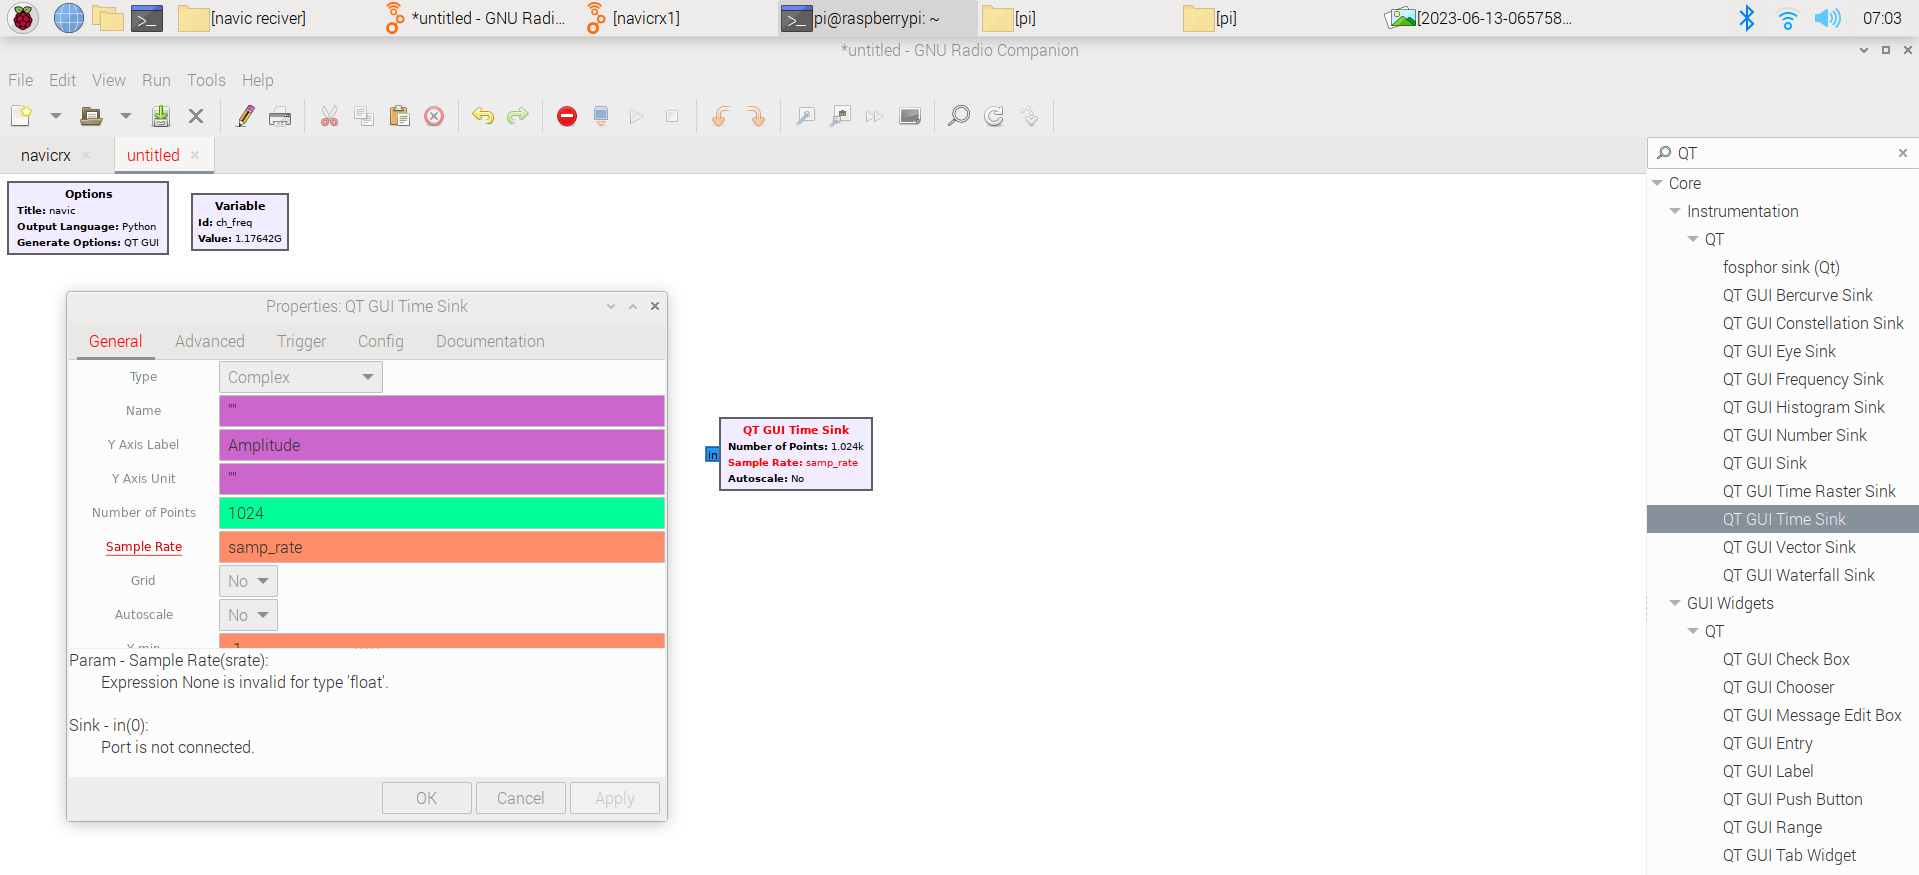
\includegraphics[width=\columnwidth]{figs/add.png}
\caption{Adding blocks}
\label{fig:add blocks}
\end{figure}
\textbf{Step-2}:
Similarly do for RTL-Source block,complex to real ,complex to imaginary and QTGUI Time sink block.
\\
\textbf{Step-3}:
Change the parameters in each block according your values by double clicking on it.
\\
\textbf{Step-4}:
Connect them according to the flowgraph shown in \figref{fig:Rx_Block_diagram}.
\begin{figure}[ht]
\centering
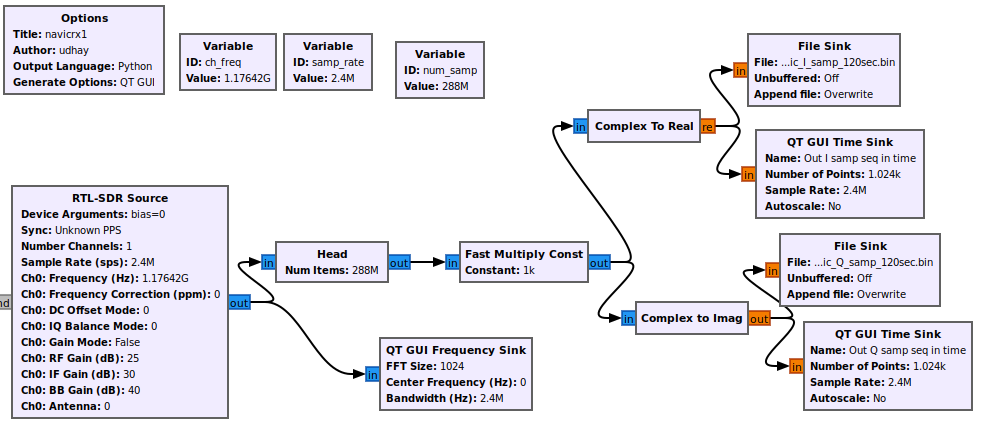
\includegraphics[width=\columnwidth]{figs/RTL_SDR_test.png}
\caption{Block diagram of Receiver in GNU Radio}
\label{fig:Rx_Block_diagram}
\end{figure}
\textbf{Note}:
Refer the following website for any queries.
\begin{lstlisting}
https://wiki.gnuradio.org/index.php?title=Creating_Your_First_Block
\end{lstlisting}
 Explain each block in block diagram of Receiver.\\
	\solution \\
\textbf{1. RTL-SDR Source}:\\
The RTL-SDR Source block is used to stream samples from RTL-SDR device.
\begin{figure}[ht]
\centering
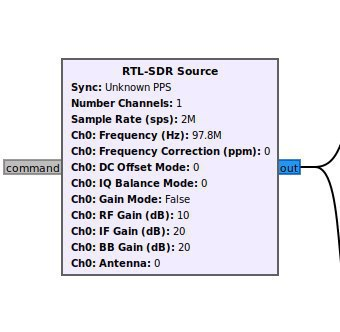
\includegraphics[width=0.4\columnwidth]{figs/source_block.png}
\caption{RTL-SDR Source Block}
\label{fig:source block_RTL}
\end{figure}
Connect the RTL-SDR to the system and execute the flowgraph in \figref{fig:Rx_Block_diagram}.\\



\subsection{Results} 
\begin{figure}
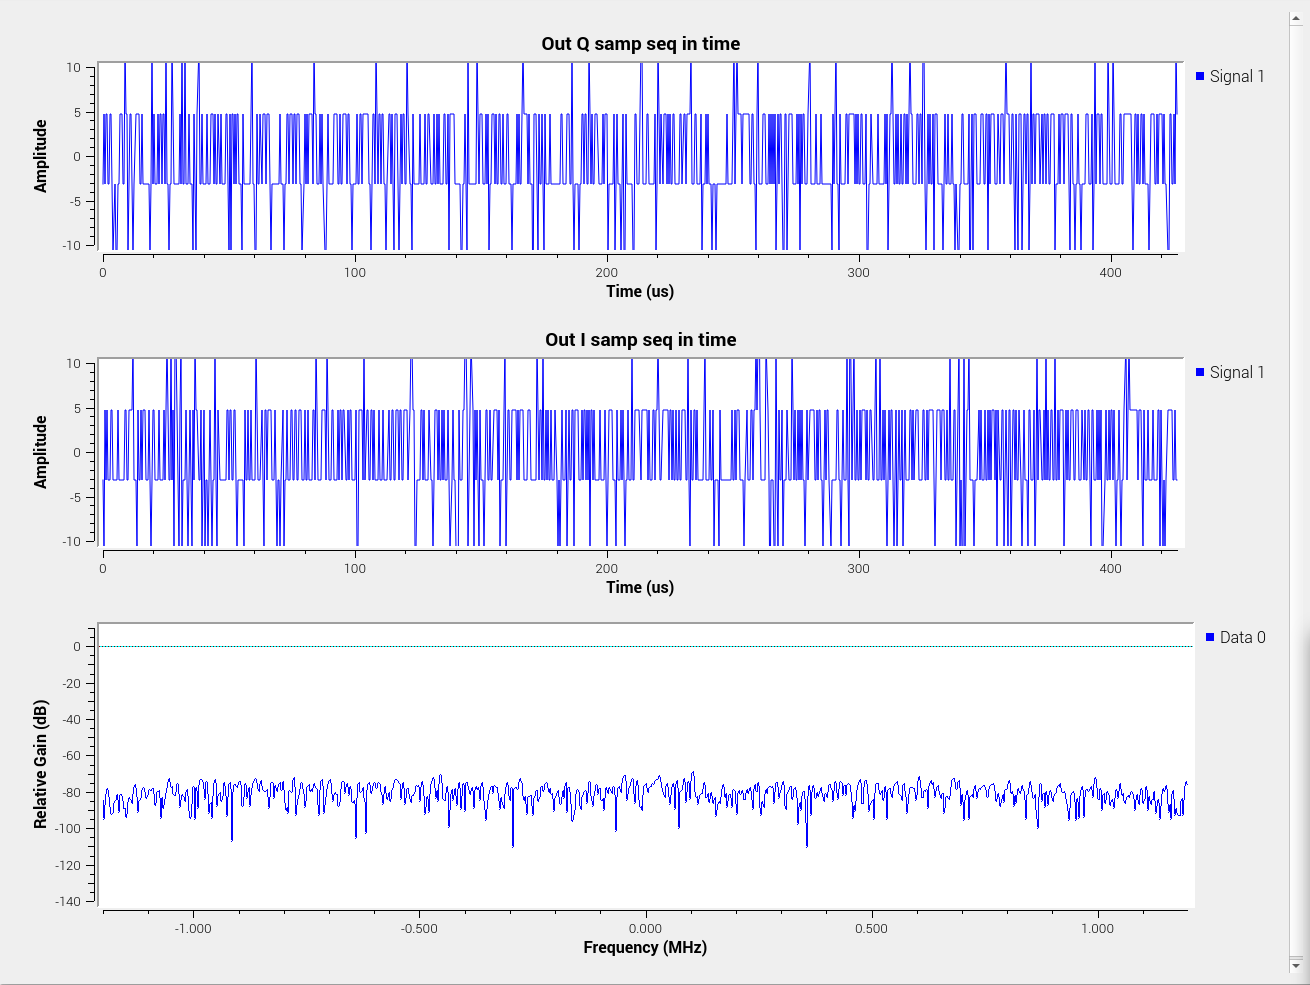
\includegraphics[width=0.8\columnwidth]{figs/RTL_sdr_res.png}
\caption{RTL-SDR receiver plots}
\end{figure}
I,Q samples will be stored in a file with .bin extension

 Read the data from RTL SDR stored in .bin file using python code and without using GNU radio.
\\
\solution \\
The following code reads the data from RTL-SDR without GNU radio.
\begin{lstlisting}
codes/receiver/rtsdr_rx.py
\end{lstlisting}














\section{USRP SDR}
The picture of Universal software Radio Peripheral-software defiend radios (USRP-SDR)  is given in \figref{fig:USRP-SDR}.This set is used to receive the L5,L1,S Band  signals.
\begin{figure}[ht]
\centering
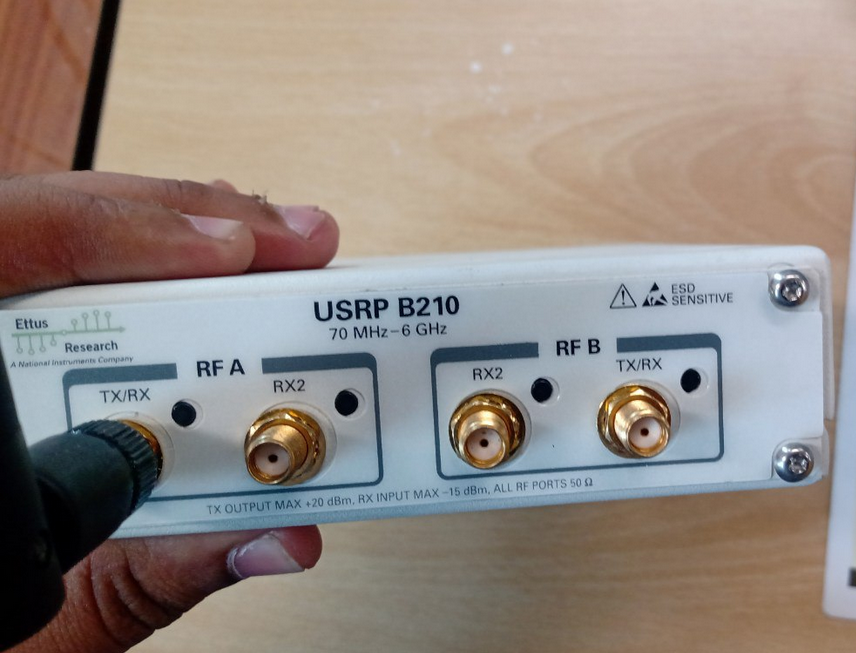
\includegraphics[width=0.5\columnwidth]{figs/USRP.png}
\caption{USRP-SDR}
\label{fig:USRP-SDR}
\end{figure}

\subsection{ USRP SDR specification}
 \begin{table}[!ht]
  \centering
 %%%%%%%%%%%%%%%%%%%%%%%%%%%%%%%%%%%%%%%%%%%%%%%%%%%%%%%%%%%%%%%%%%%%%%
%%                                                                  %%
%%  This is the header of a LaTeX2e file exported from Gnumeric.    %%
%%                                                                  %%
%%  This file can be compiled as it stands or included in another   %%
%%  LaTeX document. The table is based on the longtable package so  %%
%%  the longtable options (headers, footers...) can be set in the   %%
%%  preamble section below (see PRAMBLE).                           %%
%%                                                                  %%
%%  To include the file in another, the following two lines must be %%
%%  in the including file:                                          %%
%%        \def\inputGnumericTable{}                                 %%
%%  at the beginning of the file and:                               %%
%%        \input{name-of-this-file.tex}                             %%
%%  where the table is to be placed. Note also that the including   %%
%%  file must use the following packages for the table to be        %%
%%  rendered correctly:                                             %%
%%    \usepackage[latin1]{inputenc}                                 %%
%%    \usepackage{color}                                            %%
%%    \usepackage{array}                                            %%
%%    \usepackage{longtable}                                        %%
%%    \usepackage{calc}                                             %%
%%    \usepackage{multirow}                                         %%
%%    \usepackage{hhline}                                           %%
%%    \usepackage{ifthen}                                           %%
%%  optionally (for landscape tables embedded in another document): %%
%%    \usepackage{lscape}                                           %%
%%                                                                  %%
%%%%%%%%%%%%%%%%%%%%%%%%%%%%%%%%%%%%%%%%%%%%%%%%%%%%%%%%%%%%%%%%%%%%%%



%%  This section checks if we are begin input into another file or  %%
%%  the file will be compiled alone. First use a macro taken from   %%
%%  the TeXbook ex 7.7 (suggestion of Han-Wen Nienhuys).            %%
\def\ifundefined#1{\expandafter\ifx\csname#1\endcsname\relax}


%%  Check for the \def token for inputed files. If it is not        %%
%%  defined, the file will be processed as a standalone and the     %%
%%  preamble will be used.                                          %%
\ifundefined{inputGnumericTable}

%%  We must be able to close or not the document at the end.        %%
	\def\gnumericTableEnd{\end{document}}


%%%%%%%%%%%%%%%%%%%%%%%%%%%%%%%%%%%%%%%%%%%%%%%%%%%%%%%%%%%%%%%%%%%%%%
%%                                                                  %%
%%  This is the PREAMBLE. Change these values to get the right      %%
%%  paper size and other niceties.                                  %%
%%                                                                  %%
%%%%%%%%%%%%%%%%%%%%%%%%%%%%%%%%%%%%%%%%%%%%%%%%%%%%%%%%%%%%%%%%%%%%%%

	\documentclass[12pt%
			  %,landscape%
                    ]{report}
       \usepackage[latin1]{inputenc}
       \usepackage{fullpage}
       \usepackage{color}
       \usepackage{array}
       \usepackage{longtable}
       \usepackage{calc}
       \usepackage{multirow}
       \usepackage{hhline}
       \usepackage{ifthen}

	\begin{document}


%%  End of the preamble for the standalone. The next section is for %%
%%  documents which are included into other LaTeX2e files.          %%
\else

%%  We are not a stand alone document. For a regular table, we will %%
%%  have no preamble and only define the closing to mean nothing.   %%
    \def\gnumericTableEnd{}

%%  If we want landscape mode in an embedded document, comment out  %%
%%  the line above and uncomment the two below. The table will      %%
%%  begin on a new page and run in landscape mode.                  %%
%       \def\gnumericTableEnd{\end{landscape}}
%       \begin{landscape}


%%  End of the else clause for this file being \input.              %%
\fi

%%%%%%%%%%%%%%%%%%%%%%%%%%%%%%%%%%%%%%%%%%%%%%%%%%%%%%%%%%%%%%%%%%%%%%
%%                                                                  %%
%%  The rest is the gnumeric table, except for the closing          %%
%%  statement. Changes below will alter the table's appearance.     %%
%%                                                                  %%
%%%%%%%%%%%%%%%%%%%%%%%%%%%%%%%%%%%%%%%%%%%%%%%%%%%%%%%%%%%%%%%%%%%%%%

\providecommand{\gnumericmathit}[1]{#1} 
%%  Uncomment the next line if you would like your numbers to be in %%
%%  italics if they are italizised in the gnumeric table.           %%
%\renewcommand{\gnumericmathit}[1]{\mathit{#1}}
\providecommand{\gnumericPB}[1]%
{\let\gnumericTemp=\\#1\let\\=\gnumericTemp\hspace{0pt}}
 \ifundefined{gnumericTableWidthDefined}
        \newlength{\gnumericTableWidth}
        \newlength{\gnumericTableWidthComplete}
        \newlength{\gnumericMultiRowLength}
        \global\def\gnumericTableWidthDefined{}
 \fi
%% The following setting protects this code from babel shorthands.  %%
 \ifthenelse{\isundefined{\languageshorthands}}{}{\languageshorthands{english}}
%%  The default table format retains the relative column widths of  %%
%%  gnumeric. They can easily be changed to c, r or l. In that case %%
%%  you may want to comment out the next line and uncomment the one %%
%%  thereafter                                                      %%
\providecommand\gnumbox{\makebox[0pt]}
%%\providecommand\gnumbox[1][]{\makebox}

%% to adjust positions in multirow situations                       %%
\setlength{\bigstrutjot}{\jot}
\setlength{\extrarowheight}{\doublerulesep}

%%  The \setlongtables command keeps column widths the same across  %%
%%  pages. Simply comment out next line for varying column widths.  %%
\setlongtables

\setlength\gnumericTableWidth{%
	95pt+%
	180pt+%
0pt}
\def\gumericNumCols{2}
\setlength\gnumericTableWidthComplete{\gnumericTableWidth+%
         \tabcolsep*\gumericNumCols*2+\arrayrulewidth*\gumericNumCols}
\ifthenelse{\lengthtest{\gnumericTableWidthComplete > \linewidth}}%
         {\def\gnumericScale{\ratio{\linewidth-%
                        \tabcolsep*\gumericNumCols*2-%
                        \arrayrulewidth*\gumericNumCols}%
{\gnumericTableWidth}}}%
{\def\gnumericScale{1}}

%%%%%%%%%%%%%%%%%%%%%%%%%%%%%%%%%%%%%%%%%%%%%%%%%%%%%%%%%%%%%%%%%%%%%%
%%                                                                  %%
%% The following are the widths of the various columns. We are      %%
%% defining them here because then they are easier to change.       %%
%% Depending on the cell formats we may use them more than once.    %%
%%                                                                  %%
%%%%%%%%%%%%%%%%%%%%%%%%%%%%%%%%%%%%%%%%%%%%%%%%%%%%%%%%%%%%%%%%%%%%%%

\ifthenelse{\isundefined{\gnumericColA}}{\newlength{\gnumericColA}}{}\settowidth{\gnumericColA}{\begin{tabular}{@{}p{95pt*\gnumericScale}@{}}x\end{tabular}}
\ifthenelse{\isundefined{\gnumericColB}}{\newlength{\gnumericColB}}{}\settowidth{\gnumericColB}{\begin{tabular}{@{}p{180pt*\gnumericScale}@{}}x\end{tabular}}

\begin{longtable}[c]{%
	b{\gnumericColA}%
	b{\gnumericColB}%
	}

%%%%%%%%%%%%%%%%%%%%%%%%%%%%%%%%%%%%%%%%%%%%%%%%%%%%%%%%%%%%%%%%%%%%%%
%%  The longtable options. (Caption, headers... see Goosens, p.124) %%
%	\caption{The Table Caption.}             \\	%
% \hline	% Across the top of the table.
%%  The rest of these options are table rows which are placed on    %%
%%  the first, last or every page. Use \multicolumn if you want.    %%

%%  Header for the first page.                                      %%
%	\multicolumn{2}{c}{The First Header} \\ \hline 
%	\multicolumn{1}{c}{colTag}	%Column 1
%	&\multicolumn{1}{c}{colTag}	\\ \hline %Last column
%	\endfirsthead

%%  The running header definition.                                  %%
%	\hline
%	\multicolumn{2}{l}{\ldots\small\slshape continued} \\ \hline
%	\multicolumn{1}{c}{colTag}	%Column 1
%	&\multicolumn{1}{c}{colTag}	\\ \hline %Last column
%	\endhead

%%  The running footer definition.                                  %%
%	\hline
%	\multicolumn{2}{r}{\small\slshape continued\ldots} \\
%	\endfoot

%%  The ending footer definition.                                   %%
%	\multicolumn{2}{c}{That's all folks} \\ \hline 
%	\endlastfoot
%%%%%%%%%%%%%%%%%%%%%%%%%%%%%%%%%%%%%%%%%%%%%%%%%%%%%%%%%%%%%%%%%%%%%%

\hhline{|-|-}
	 \multicolumn{1}{|p{\gnumericColA}|}%
	{\gnumericPB{\raggedright}\gnumbox[l]{\hspace{0.75cm}\textbf{Name}}}
	&\multicolumn{1}{p{\gnumericColB}|}%
	{\gnumericPB{\raggedright}\gnumbox[l]{ \textbf{USRP B210}}}
\\
\hhline{|--|}
	 \multicolumn{1}{|p{\gnumericColA}|}%
	{\gnumericPB{\raggedright}\gnumbox[l]{Type}}
	&\multicolumn{1}{p{\gnumericColB}|}%
	{\gnumericPB{\raggedright}\gnumbox[l]{Pre-built}}
\\
\hhline{|--|}
	 \multicolumn{1}{|p{\gnumericColA}|}%
	{\gnumericPB{\raggedright}\gnumbox[l]{Frequency range}}
	&\multicolumn{1}{p{\gnumericColB}|}%
	{\gnumericPB{\raggedright}\gnumbox[l]{70MHz-6GHz}}
\\
\hhline{|--|}
	 \multicolumn{1}{|p{\gnumericColA}|}%
	{\gnumericPB{\raggedright}\gnumbox[l]{Max Bandwidth}}
	&\multicolumn{1}{p{\gnumericColB}|}%
	{\gnumericPB{\raggedright}\gnumbox[l]{56MHz}}
\\
\hhline{|--|}
	 \multicolumn{1}{|p{\gnumericColA}|}%
	{\gnumericPB{\raggedright}\gnumbox[l]{Receiver ADC bits }}
	&\multicolumn{1}{p{\gnumericColB}|}%
	{\gnumericPB{\raggedright}\gnumbox[l]{12}}
\\
\hhline{|--|}
	 \multicolumn{1}{|p{\gnumericColA}|}%
	{\gnumericPB{\raggedright}\gnumbox[l]{Tx.DAC bits}}
	&\multicolumn{1}{p{\gnumericColB}|}%
	{\gnumericPB{\raggedright}\gnumbox[l]{12}}
\\
\hhline{|--|}
	 \multicolumn{1}{|p{\gnumericColA}|}%
	{\gnumericPB{\raggedright}\gnumbox[l]{Tx. Cable }}
	&\multicolumn{1}{p{\gnumericColB}|}%
	{\gnumericPB{\raggedright}\gnumbox[l]{Yes}}
\\
\hhline{|--|}
	 \multicolumn{1}{|p{\gnumericColA}|}%
	{\gnumericPB{\raggedright}\gnumbox[l]{Sampling Rate }}
	&\multicolumn{1}{p{\gnumericColB}|}%
	{\gnumericPB{\raggedright}\gnumbox[l]{50 Msps }}
\\
\hhline{|-|-|}
\multicolumn{1}{|p{\gnumericColA}|}%
	{\gnumericPB{\raggedright}\gnumbox[l]{Frequency accuracy }}
	&\multicolumn{1}{p{\gnumericColB}|}%
	{\gnumericPB{\raggedright}\gnumbox[l]{-}}
\\
\hhline{|--|}
	 \multicolumn{1}{|p{\gnumericColA}|}%
	{\gnumericPB{\raggedright}\gnumbox[l]{Host inerface }}
	&\multicolumn{1}{p{\gnumericColB}|}%
	{\gnumericPB{\raggedright}\gnumbox[l]{USB 3.0 }}
\\
\hhline{|--|}
	 \multicolumn{1}{|p{\gnumericColA}|}%
	{\gnumericPB{\raggedright}\gnumbox[l]{FPGA}}
	&\multicolumn{1}{p{\gnumericColB}|}%
	{\gnumericPB{\raggedright}\gnumbox[l]{ Xilinx Spartan 6 XC6SLX150}}
\\

\hhline{|--|}
\end{longtable}

\ifthenelse{\isundefined{\languageshorthands}}{}{\languageshorthands{\languagename}}
\gnumericTableEnd

 \caption{USRP-SDR Specification table }
\end{table}

 Install and open GNU Radio using the following commands
\\
\begin{lstlisting}
sudo apt update
sudo apt install gnuradio
gnuradio-companion
\end{lstlisting}
 How to construct the block diagram in GNU radio? \\
	\solution  \\
\textbf{Step-1}:\\
Search for QTGUI Time sink  block and add it to the work space.
\begin{figure}[H]
\centering
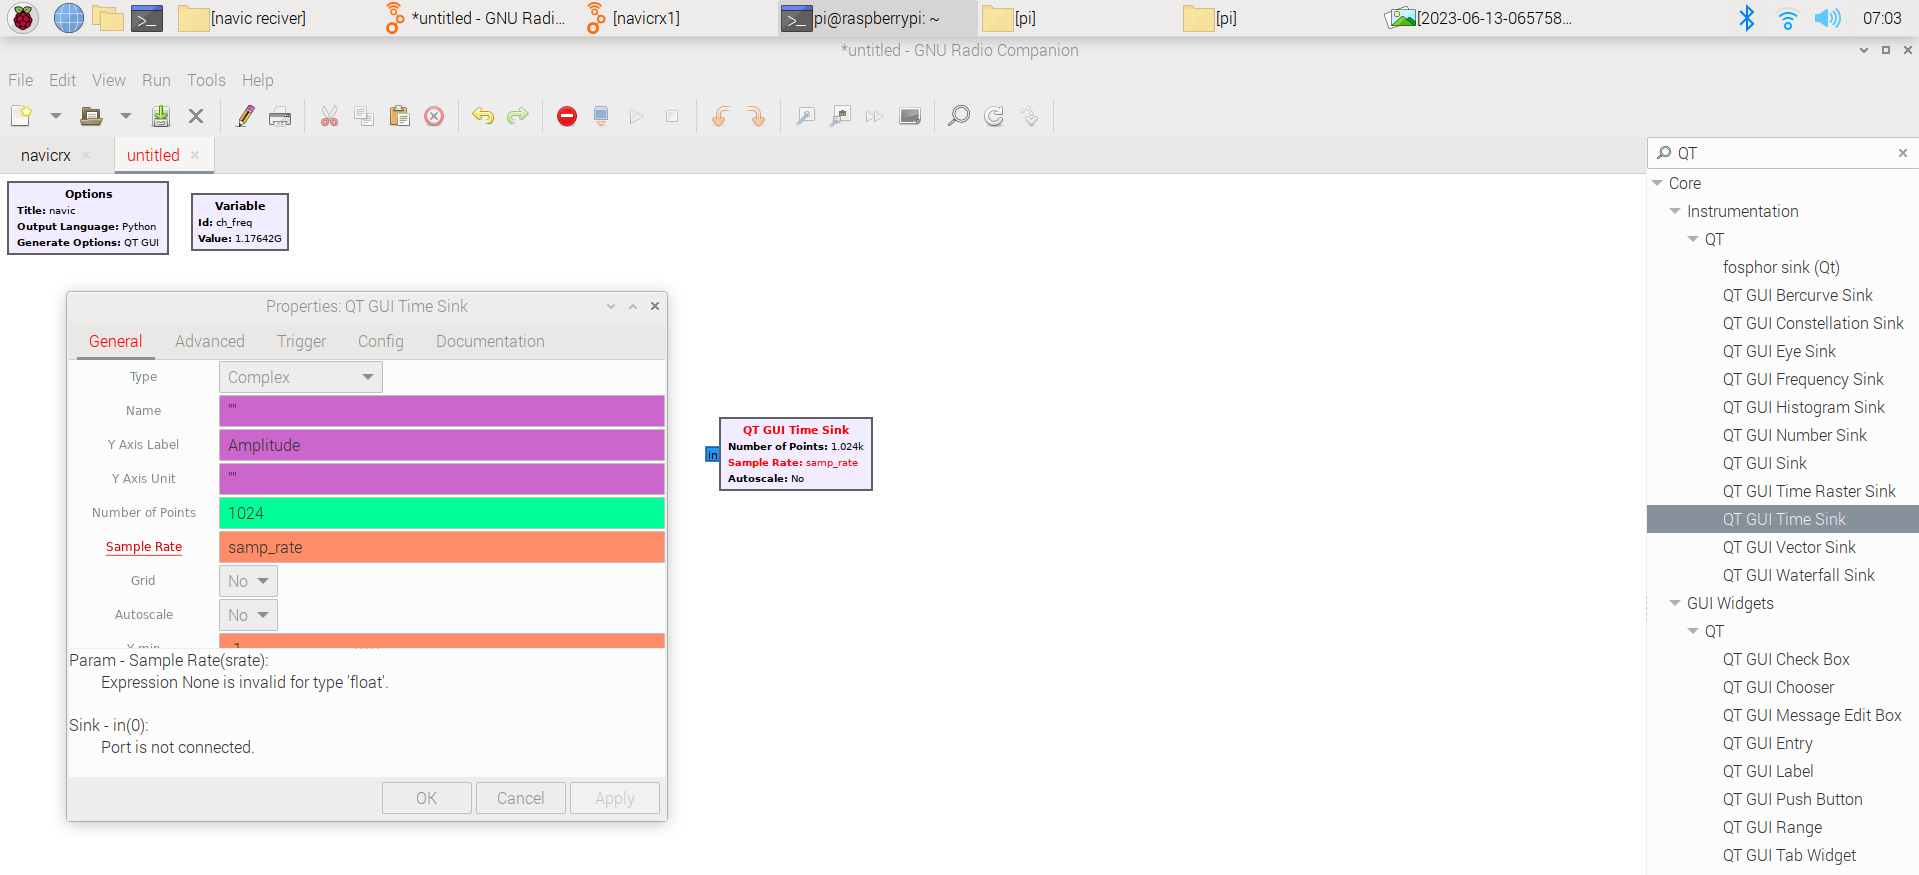
\includegraphics[width=\columnwidth]{figs/add.png}
\caption{Adding blocks}
\label{fig:adding blocks}
\end{figure}
\textbf{Step-2}:
Similarly do for USRP-Source block,complex to real ,complex to imaginary and QTGUI Time sink block.
\\
\textbf{Step-3}:
Change the parameters in each block according your values by double clicking on it.
\\
\textbf{Step-4}:
Connect them according to the flowgraph shown in \figref{fig:Rx_Block_diagram}.
\begin{figure}[H]
\centering
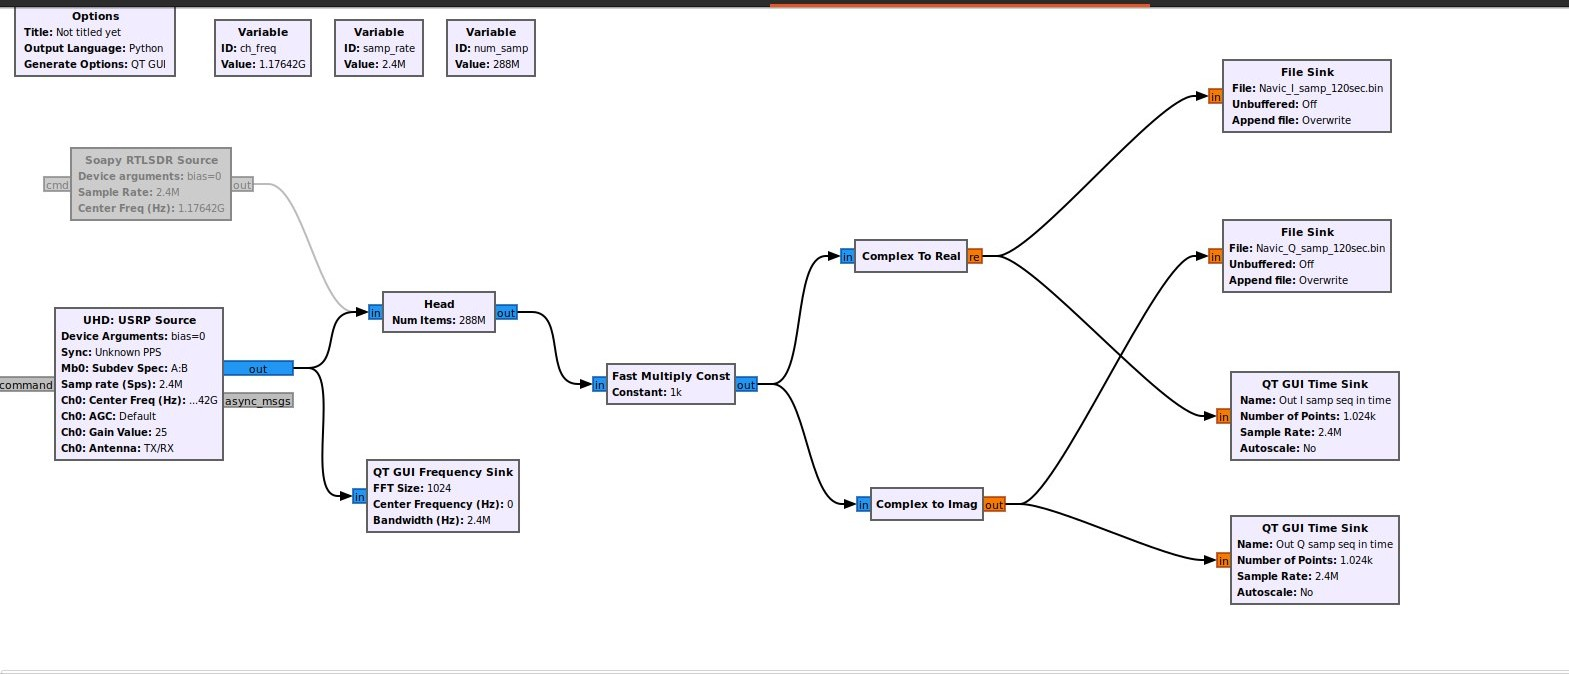
\includegraphics[width=\columnwidth]{figs/USRP_navic.jpg}
\caption{Block diagram of Receiver in GNU Radio}
\label{fig:Rx_Block_diagram_USRP}
\end{figure}
\textbf{Note}:
Refer the following website for any queries.
\begin{lstlisting}
https://wiki.gnuradio.org/index.php?title=Creating_Your_First_Block
\end{lstlisting}
 Explain each block in block diagram of Receiver.\\
	\solution \\
\textbf{1. RTL-SDR Source}:\\
The RTL-SDR Source block is used to stream samples from USRP-SDR device.
\begin{figure}[H]
\centering
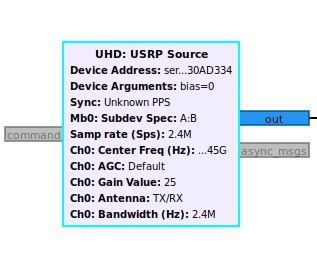
\includegraphics[width=0.4\columnwidth]{figs/usrp-sink.jpg}
\caption{USRP-SDR Source Block}
\label{fig:source block_USRP}
\end{figure}
Connect the USRP-SDR as shown flowgraph in \figref{fig:Rx_Block_diagram_USRP}.\\



\subsection{Results} 
\begin{figure}
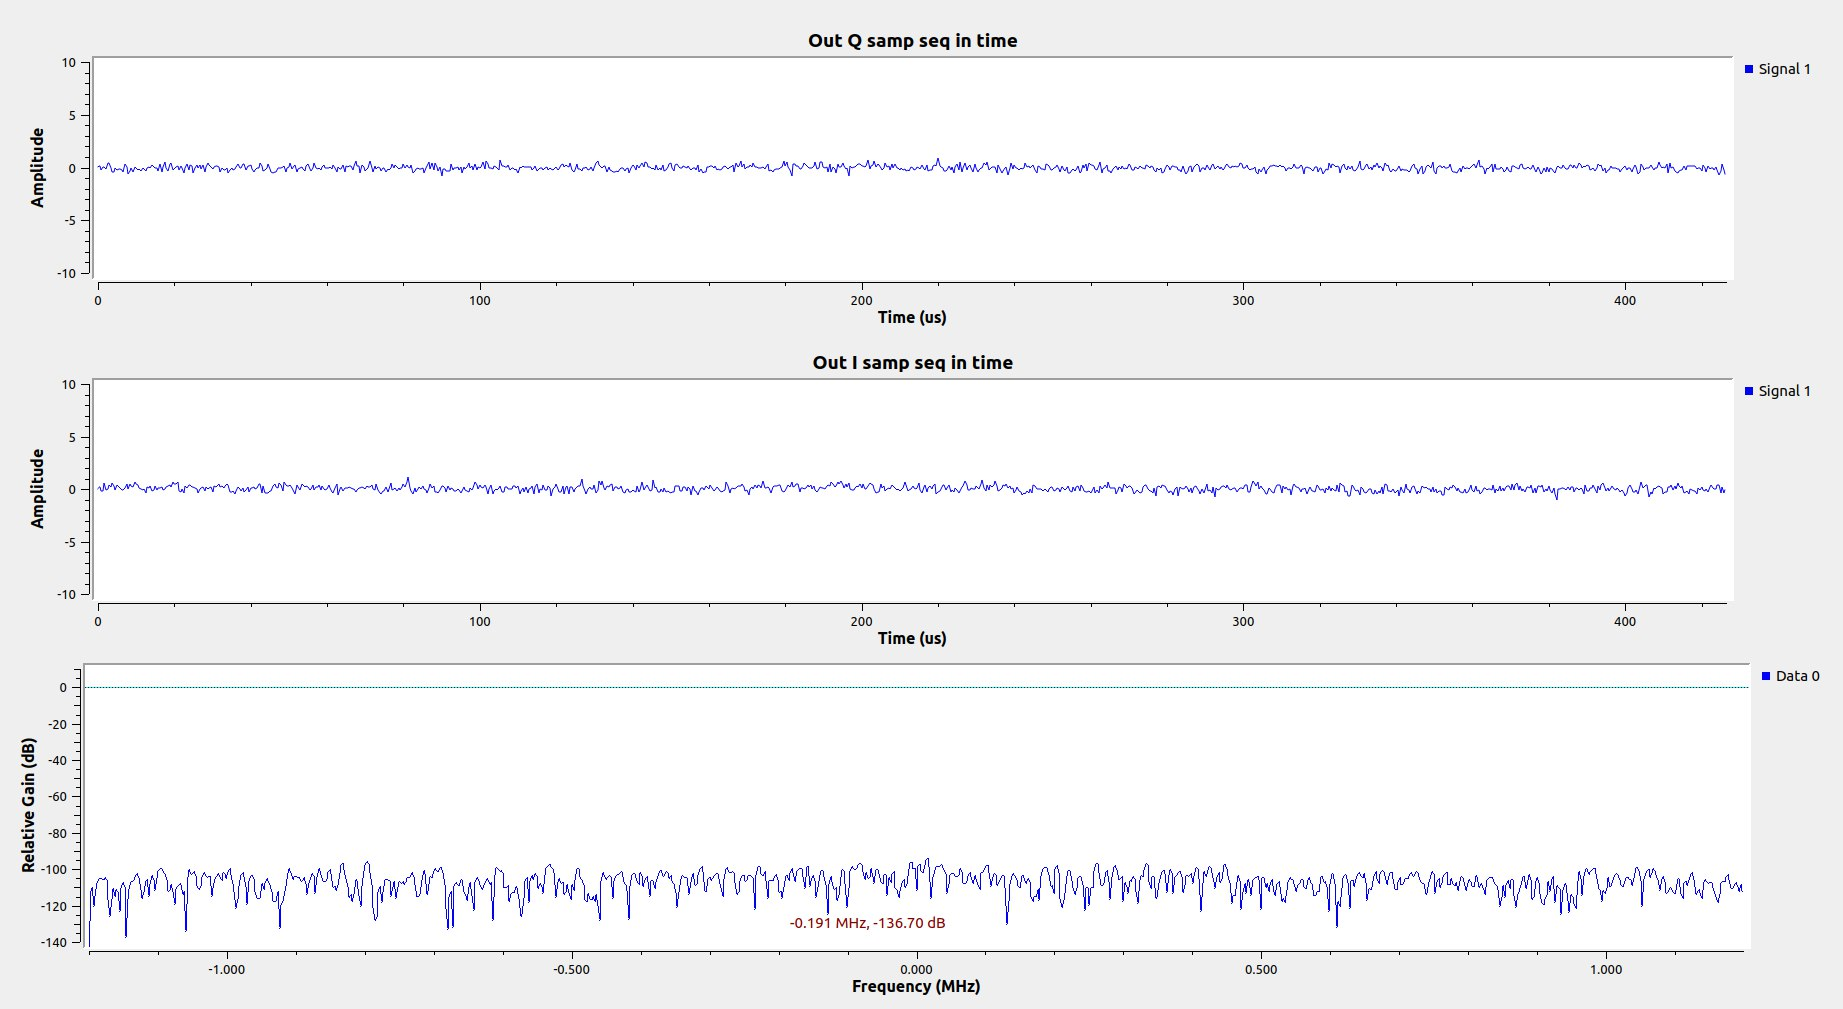
\includegraphics[width=0.8\columnwidth]{figs/USRP_results.jpg}
\caption{USRP receiver plots}
\label{fig:plots}
\end{figure}

I,Q samples will be stored in a file with .bin extension

Read the data from RTL SDR stored in .bin file using python code and without using GNU radio.
\\
\solution \\
The following code reads the data from RTL-SDR without GNU radio.
\begin{lstlisting}
codes/receiver/usrp_rx.py
\end{lstlisting}
















